\documentclass{article}
\usepackage{hyperref}
\usepackage{amsmath,amssymb}
\usepackage{graphicx}
\usepackage{caption}
\usepackage{subcaption}

\renewcommand{\thesubsection}{\thesection.\alph{subsection}}

\title{\bf{CSE397: Assignment \#1}}
\author{Nicholas Malaya \\ Institute for Computational Engineering and Sciences \\ University of Texas at Austin} \date{}

\begin{document}
\maketitle

\newpage
\section{Problem 1}

\begin{figure}[p]
  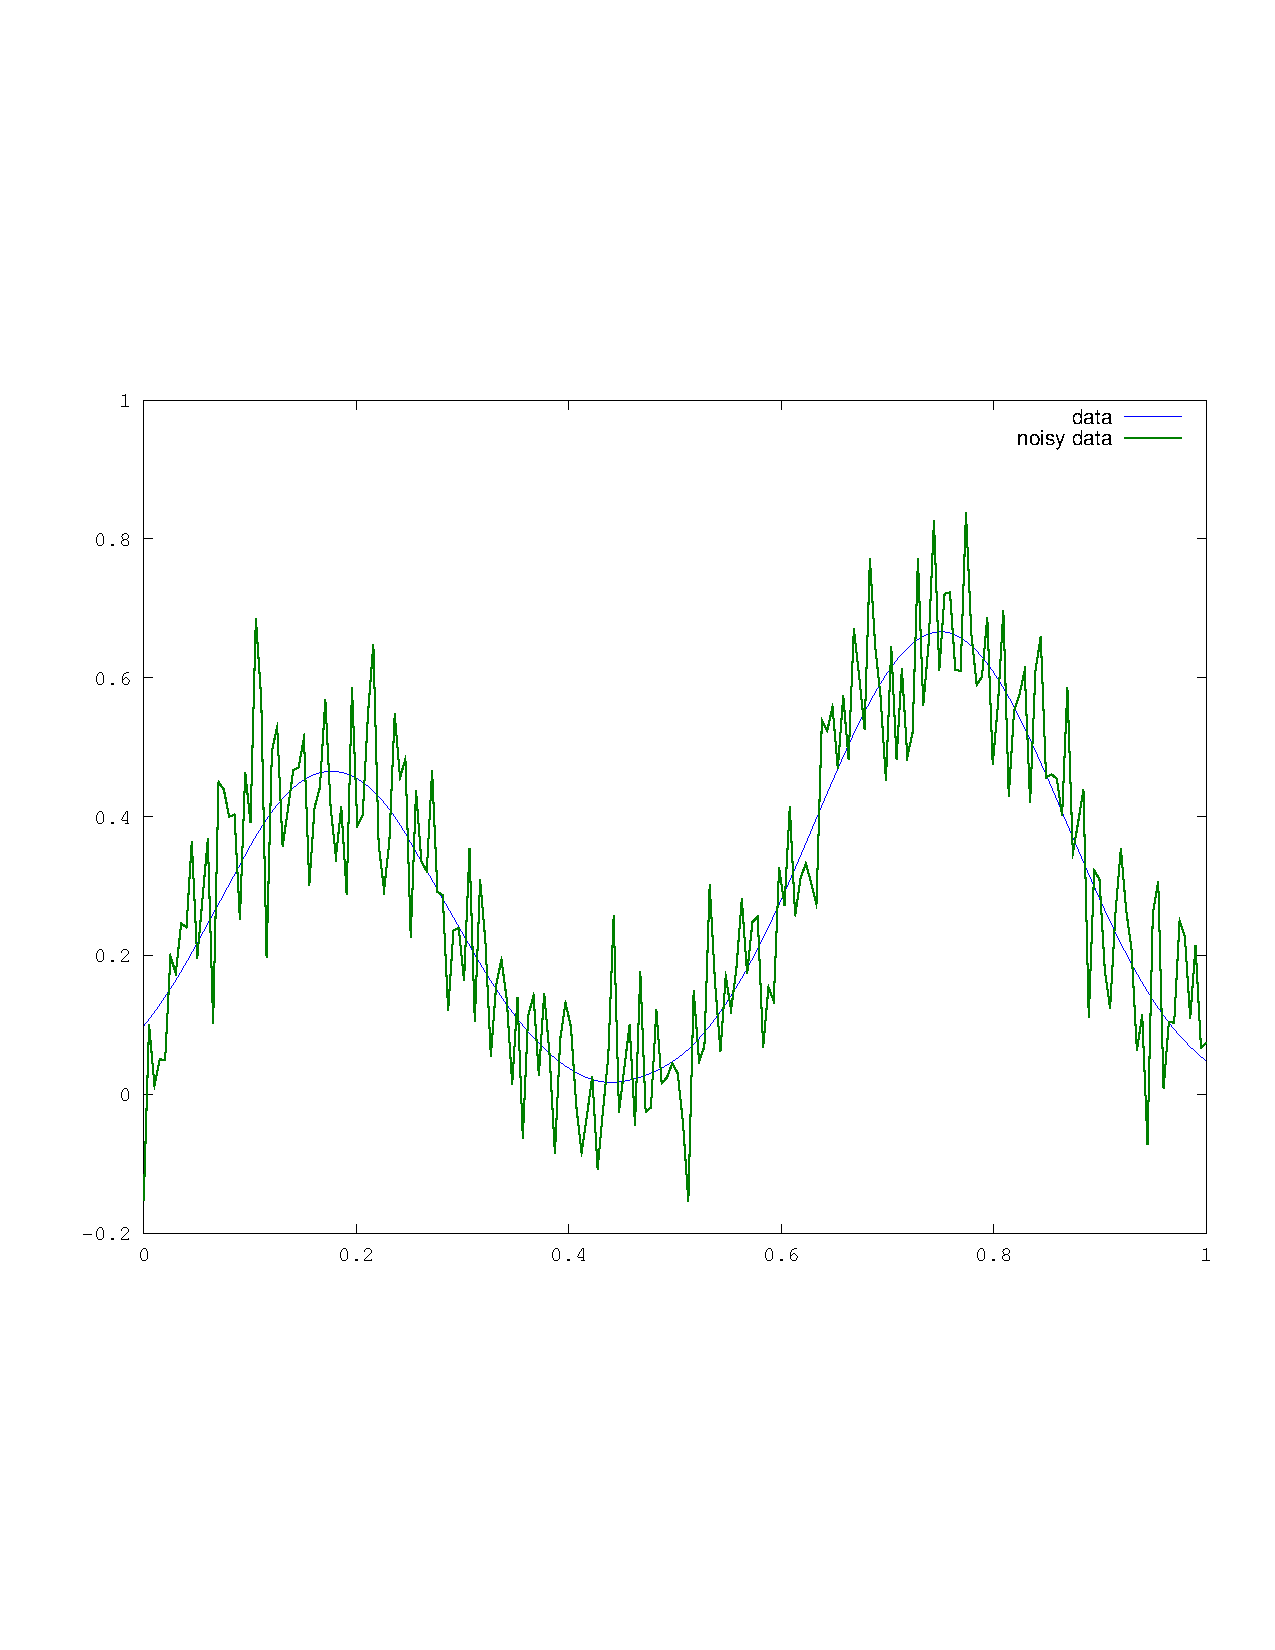
\includegraphics[scale=.5]{plots/data.pdf}
  \label{fig:data}
  \caption{The data (after applying the filter) with and without
 normally distributed noise. } 
\end{figure}

After applying the new filter $k(x)$ and adding gaussian noise, the data
used as input for the inverse problem is plotted in figure
\ref{fig:data}. 

Notice that this filter is significant: the raw data generated after
passing through the filter (even without statistical noise) has lost
several features of the underlying ``true'' signal. 

\subsection{$T_{\text{SVD}}$}



\subsection{Tikhanov Filter}

\begin{figure}
        \centering
        \begin{subfigure}[b]{0.3\textwidth}
                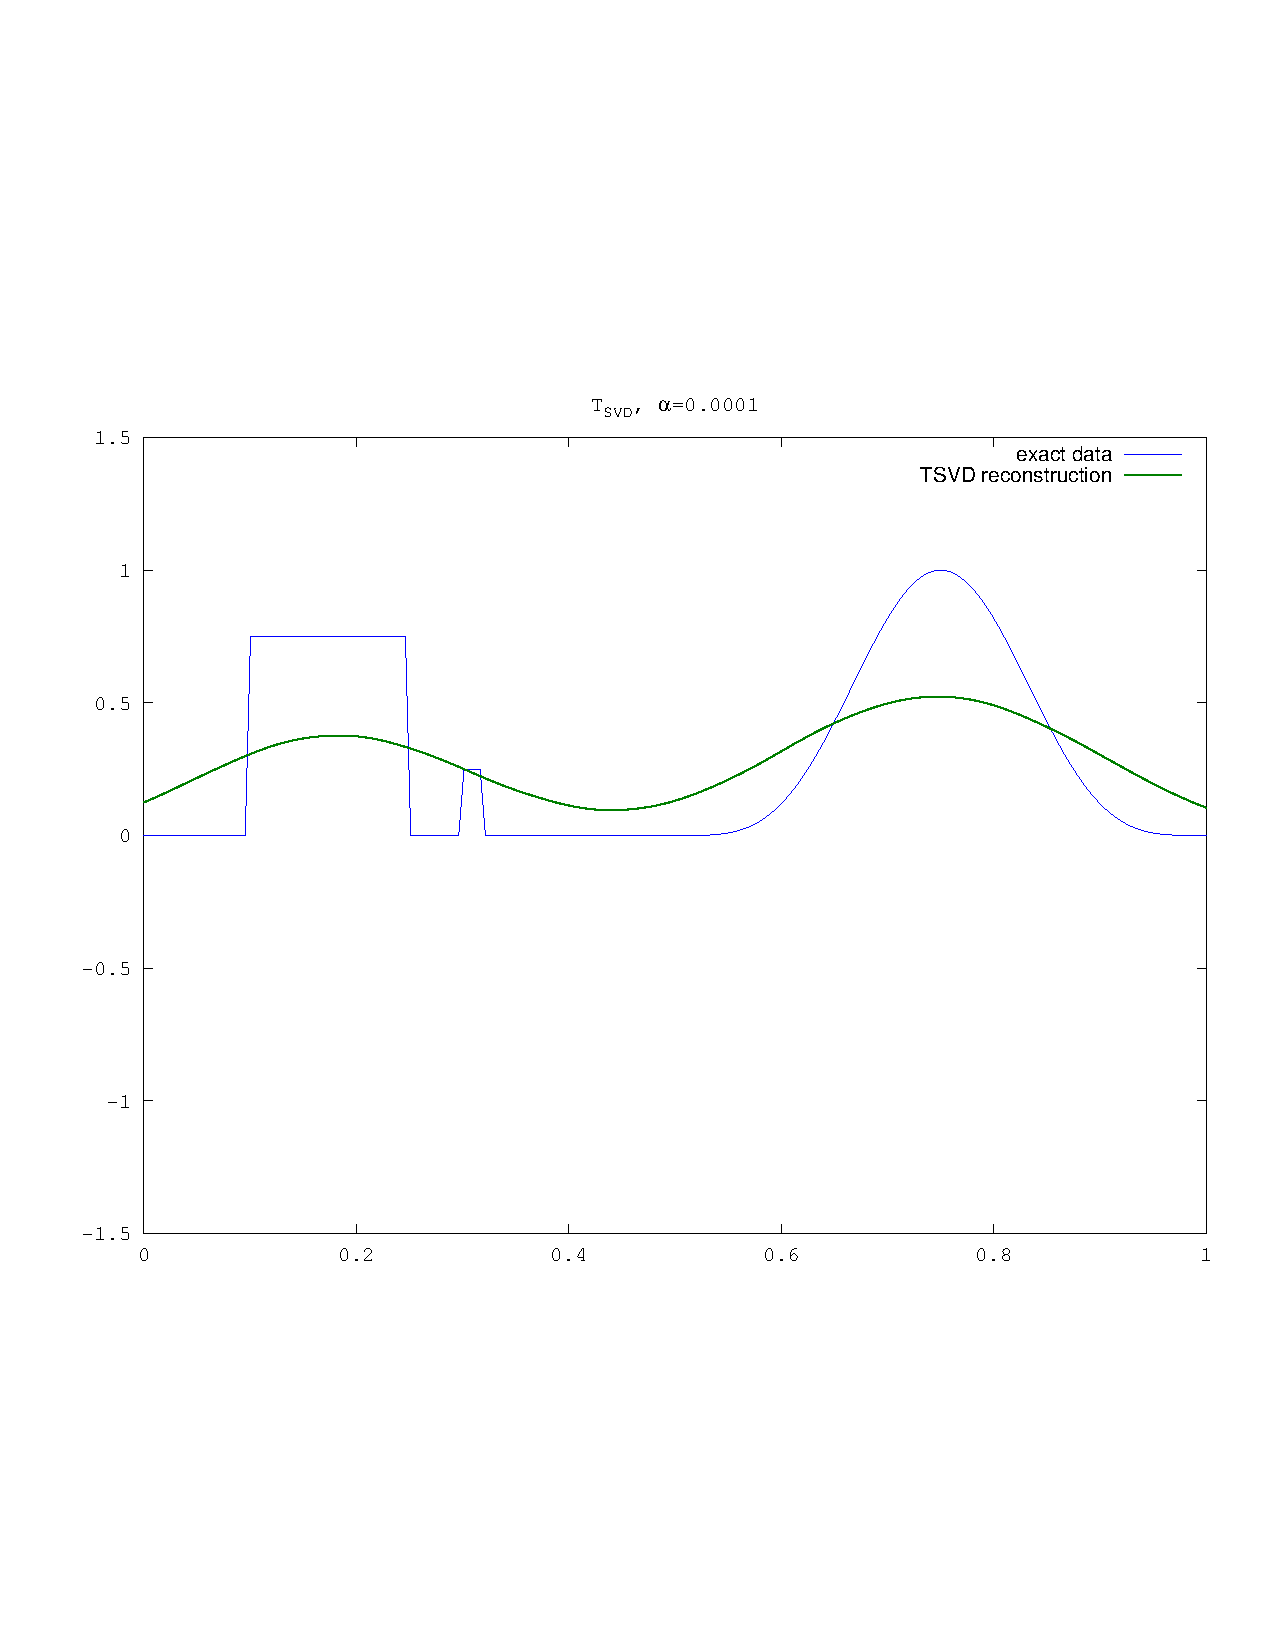
\includegraphics[width=\textwidth]{plots/tsvd0001.pdf}
                \caption{$\alpha=0.0001$}
        \end{subfigure}%
        \begin{subfigure}[b]{0.3\textwidth}
                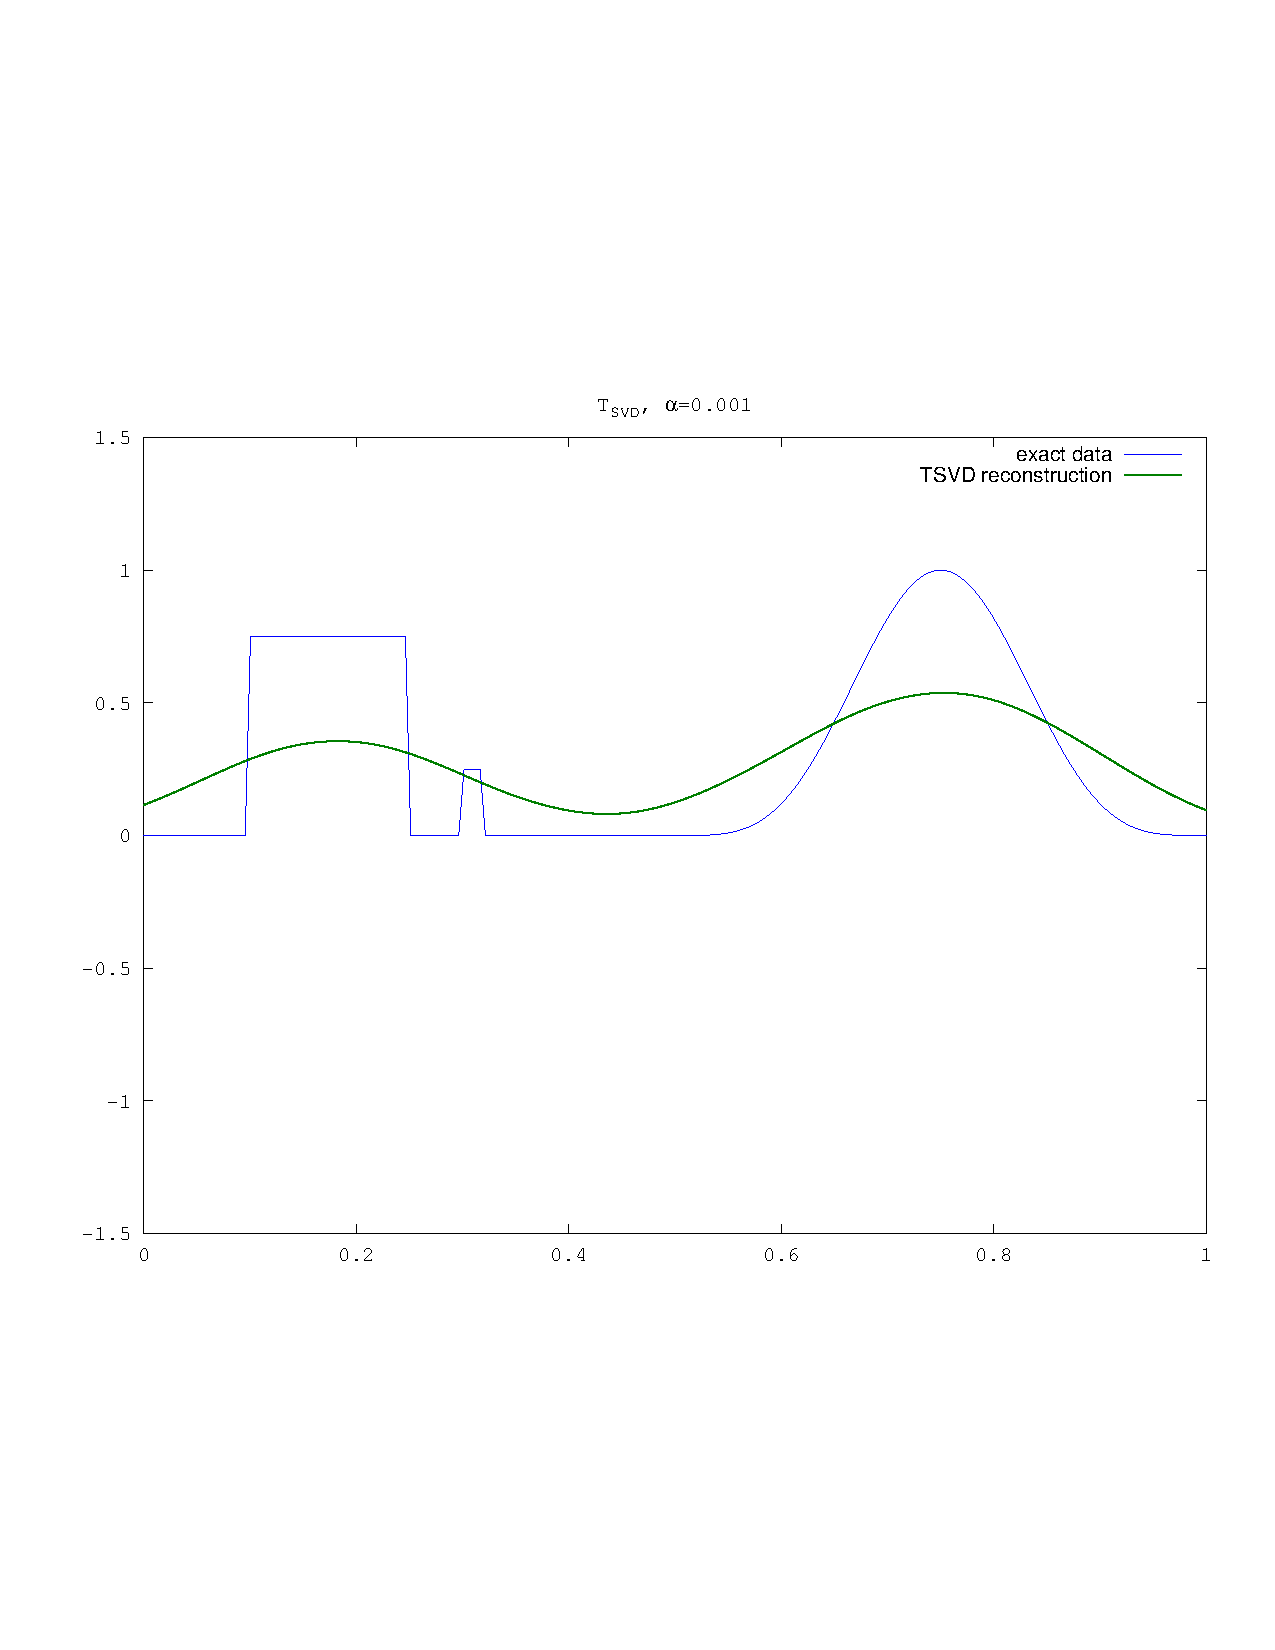
\includegraphics[width=\textwidth]{plots/tsvd001.pdf}
                \caption{$\alpha=0.001$}
        \end{subfigure}
        \centering
        \begin{subfigure}[b]{0.3\textwidth}
                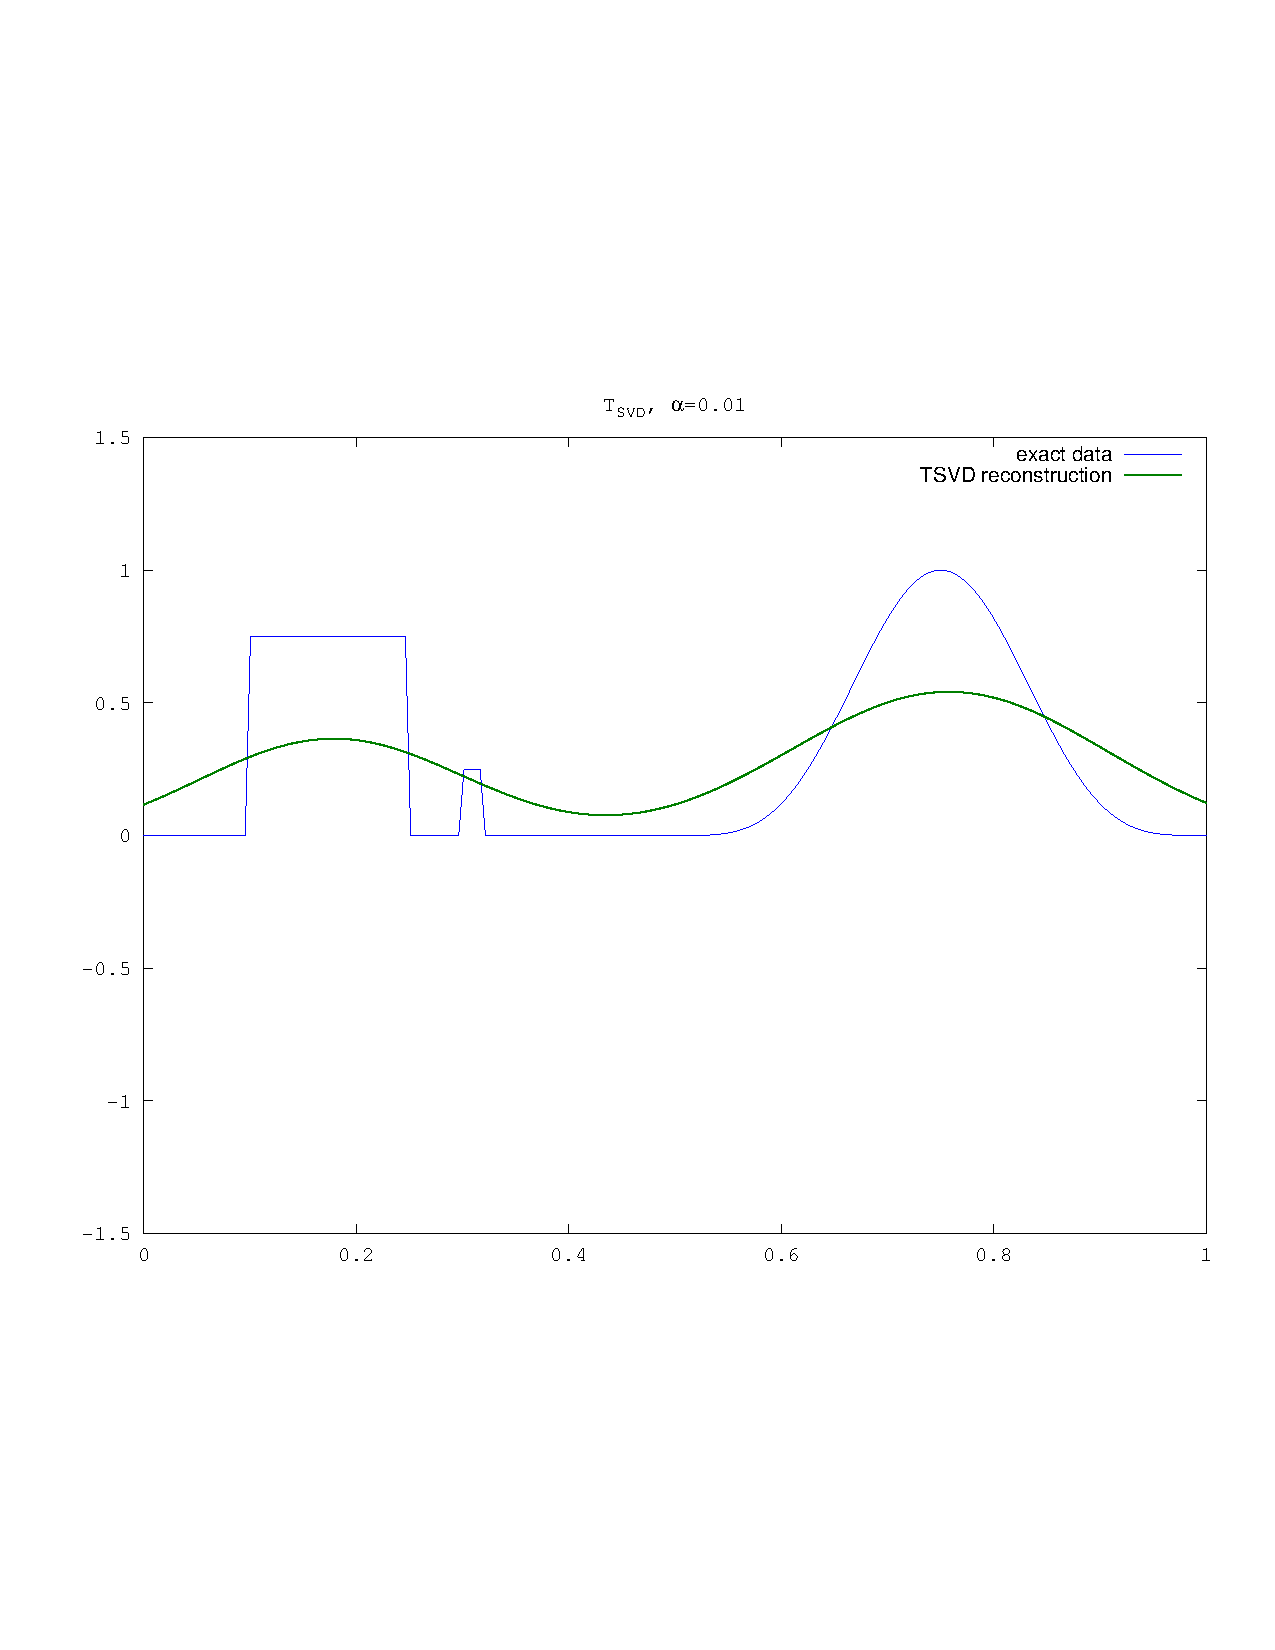
\includegraphics[width=\textwidth]{plots/tsvd01.pdf}
                \caption{$\alpha=0.1$}
        \end{subfigure}%
        \begin{subfigure}[b]{0.3\textwidth}
                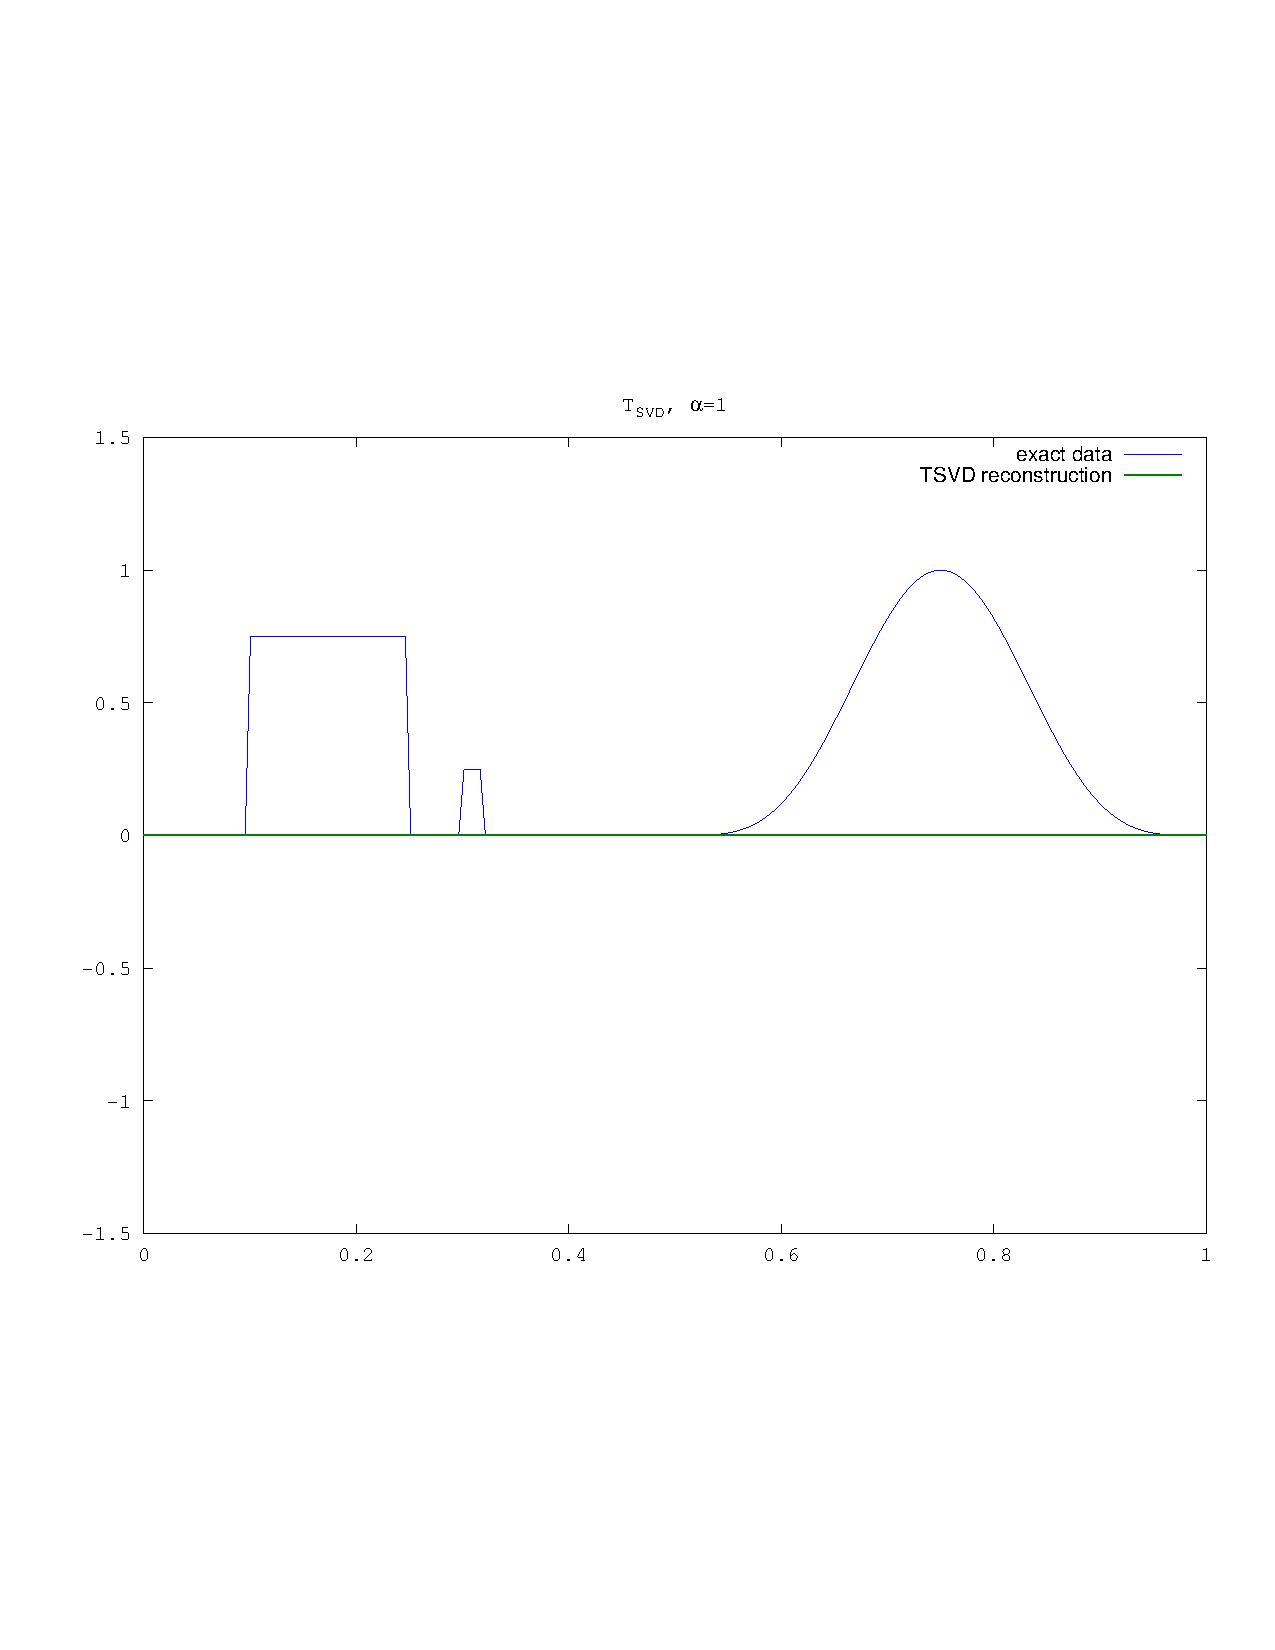
\includegraphics[width=\textwidth]{plots/tsvd1.pdf}
                \caption{$\alpha=1.0$}
        \end{subfigure}
        \caption{$T_{\text{SVD}}$ at varying values of $\alpha$.}
\end{figure}


\subsection{L-Curve}


\subsection{Morozov's Discrepancy Criterion}


\subsection{Actual Error}


\newpage
\section{Problem 2}


\subsection{Memory Requirement}


\subsection{L-Curve}


\subsection{Actual Error}

\end{document}